%%%%%%%%%%%%%%%%%%%%%%%%%%%%%%%%%%%%%%%%%%%%%%%%%%%%%%%%%%%%%%%%%%%%%%%%%%%
%% This file is part of the book
%%
%% Algorithmic Graph Theory
%% http://code.google.com/p/graph-theory-algorithms-book/
%%
%% Copyright (C) 2009, 2010, 2011 Minh Van Nguyen <nguyenminh2@gmail.com>
%%
%% See the file COPYING for copying conditions.
%%%%%%%%%%%%%%%%%%%%%%%%%%%%%%%%%%%%%%%%%%%%%%%%%%%%%%%%%%%%%%%%%%%%%%%%%%%

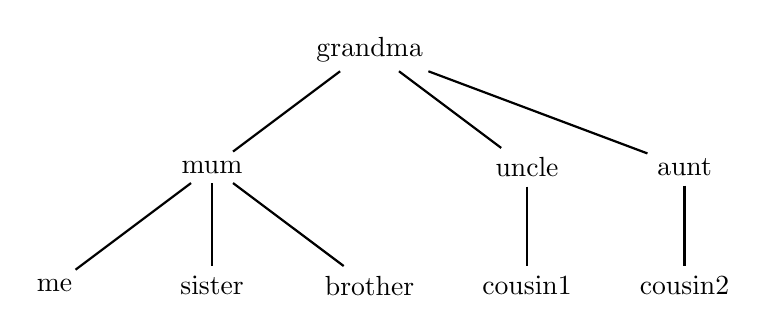
\begin{tikzpicture}
[nodedecorate/.style={shape=circle,inner sep=2pt,draw,thick},%
  linedecorate/.style={-,thick}]
%% nodes or vertices
\foreach \nodename/\x/\y in {me/0/0, sister/2/0, brother/4/0,
  mum/2/1.5, cousin1/6/0, cousin2/8/0, uncle/6/1.5, aunt/8/1.5,
  grandma/4/3}
{
  \node (\nodename) at (\x,\y) [] {\nodename};
}
%% edges or lines
\path
\foreach \startnode/\endnode in {grandma/mum, grandma/uncle,
  grandma/aunt, mum/me, mum/sister, mum/brother, uncle/cousin1,
  aunt/cousin2}
{
  (\startnode) edge[linedecorate] node {} (\endnode)
};
\end{tikzpicture}
